\chapter{实验和结果}\label{chapter:experiments}

为验证本文技术的效果,本文设计了两个实验,实验A用于验证客观评价算法的效果,实验B用于验证短波信道语音自动选路的最终效果。

实验A使用采集到的500个短波语音,分别使用客观评价算法、主观评价平台进行客观评分和主观评分。我们绘制主观评分结果和客观评分结果的线性回归图,分析客观评分和主观评分的相关关系,从而分析主观评价结果的好坏。此外我们将本文所提算法和两种标准客观评分算法的结果进行了比较。

实验B同时在多地采集同一短波信号,再使用本文的自动选路系统进行选路输出,对比最终结果语音和各路原始语音的质量,从而分析自动选路技术的效果优劣。

\section{实验数据采集}

由于没有现成的公开短波语音数据集,本文自建了一组短波语音的数据集并进行主观质量评分。
本文实验数据的采集,是使用短波收音机对各短波电台广播进行录音来获取的。在录音时使用音频线直接将短波收音机和录音笔连接起来,使用录音笔录音,从而避免引入附加的环境噪音。

对于实验A,我们在每天不同时段,对多个短波电台进行录音。然后对采集到的音频数据进行降采样,统一采样率为8kHz,再分割成每段2s的短语音,保存成“wav”格式。最终生成500个时长2s的短波语音片段。

对于实验B,由多人在2-3个城市,5-6个地点同时对同一频率的短波广播进行录音,各录音地点之间距离相隔不少于500m。对采集到的音频数据进行降采样,统一采样率为8kHz,分割成每段60s左右的语音,并保存为“wav”格式,命名形式为[时间]-[地点]-[频率]。

\section{实验A结果}

在实验A中,我们使用本文所提的两种客观评价算法分别对采集到的500个短波语音片段进行了客观质量评分。同时我们召集了16位志愿者,利用第~\ref{chapter:web}章介绍的在线辅助系统进行了主观意见分的评分。我们分别对两种算法的客观评分和主观评分进行了线性回归,作图如图~\ref{fig:regress}所示,其中每个蓝色散点代表一个语音片段,横坐标为算法客观评分结果,纵坐标为平均主观意见分,红色直线为线性回归的结果。图~\ref{fig:regress1}为基于语谱图噪音模型的算法结果,图~\ref{fig:regress2}为基于自编码器的算法结果。从图中可以看出本文所提算法给出的语音质量客观评分能够反映出其主观感受质量的好坏。

\begin{figure}
\centering
\subcaptionbox{基于语谱图噪音模型的算法\label{fig:regress1}}{
    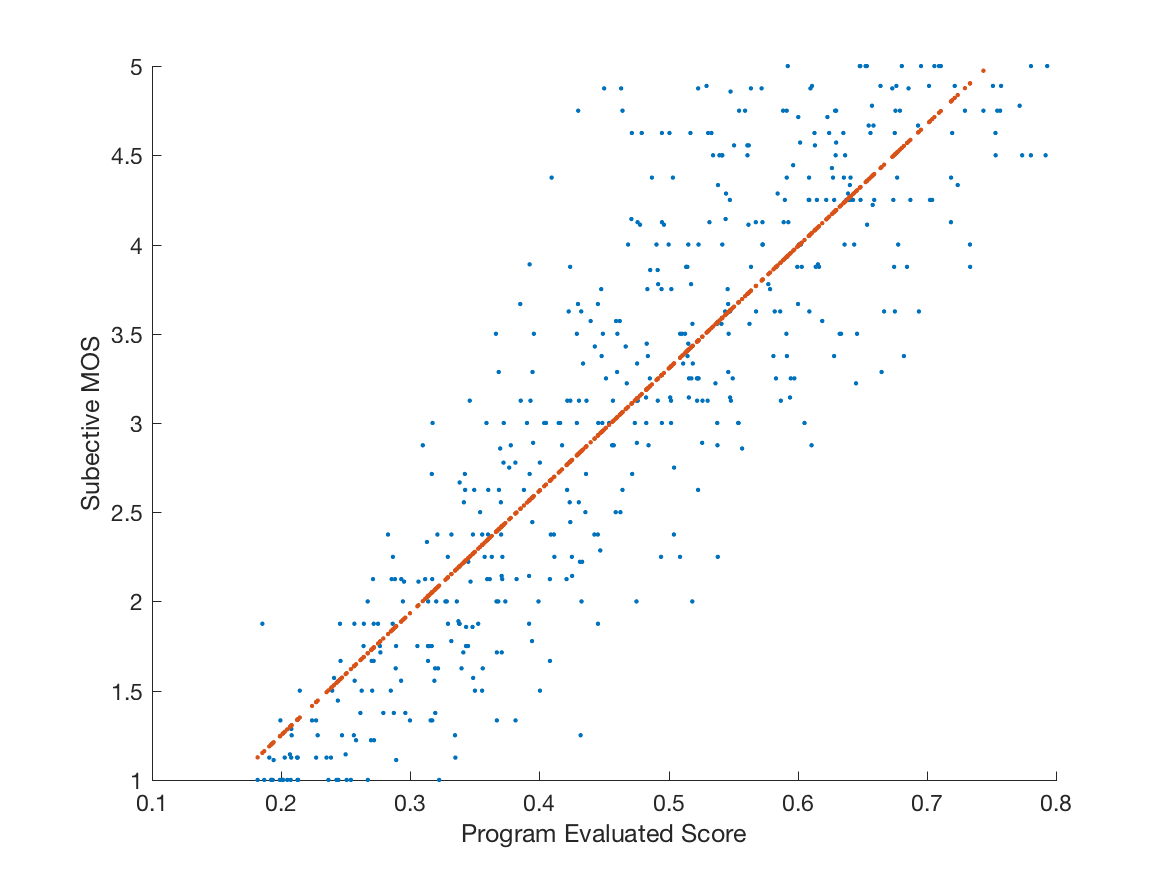
\includegraphics[width=0.45\textwidth]{regress}
}
\subcaptionbox{基于自编码器的算法\label{fig:regress2}}{
    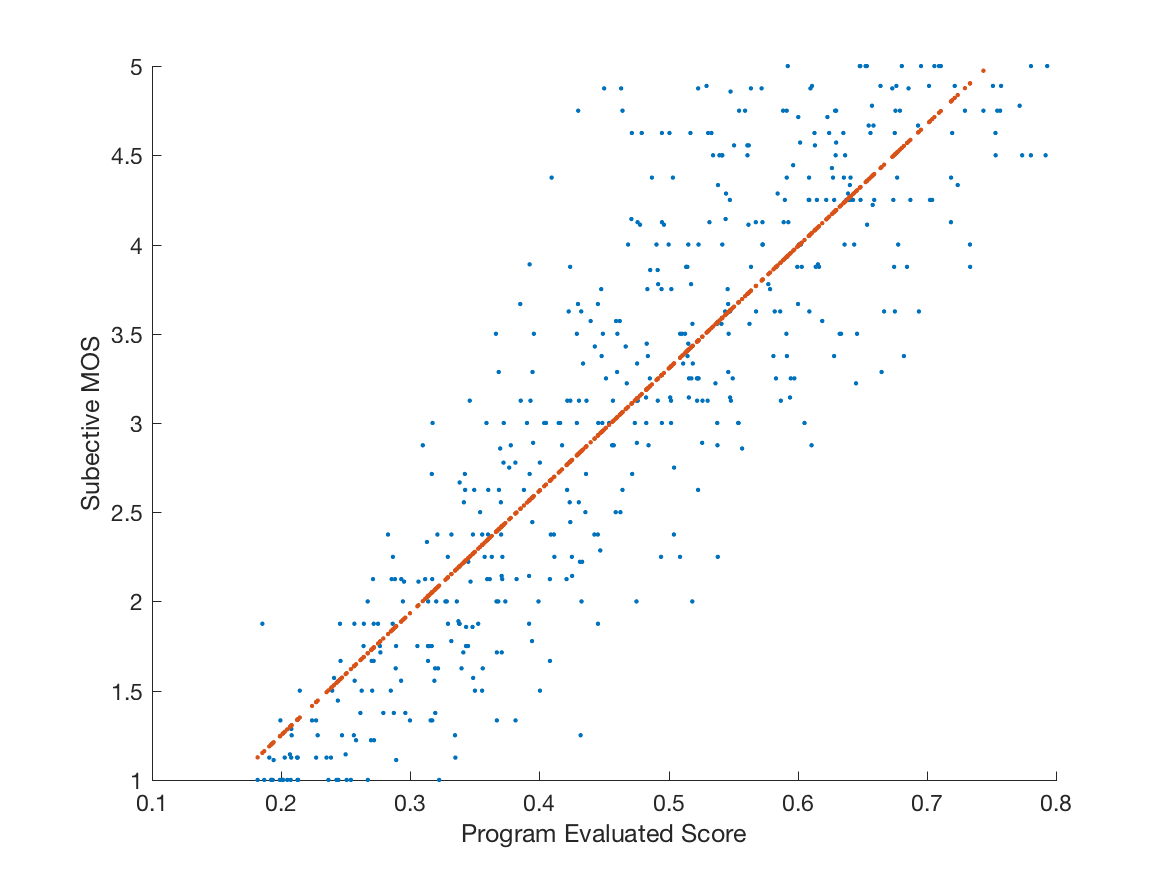
\includegraphics[width=0.45\textwidth]{regress}
}
\vspace{0.8ex}
\\
\caption{客观评分结果和平均主观意见分的线性回归\label{fig:regress}}
\end{figure}

进一步地,我们使用了两种对比算法对500个短波语音片段进行了客观质量评分。这两种对比算法分别为被ITU-T标准收录的P.563算法和被ANSI标准收录的ANIQUE+算法。我们通过一下几种评价指标来对比本文所提算法和这两种对比算法的性能。

\begin{itemize}
\item Spearman Correlation Coefficient (SCC) - 斯皮尔曼等级相关系数是衡量两个变量的相关性的非参数指标,利用单调方程评价两个统计变量的相关性,取值范围在-1到+1之间,绝对值越接近1说明两个变量相关性越高。通过计算客观评分和主观评分的斯皮尔曼等级相关系数,反应客观评分和主观评分的相关性,绝对值越接近1说明算法效果越好。
\item Root Mean Square Error (RMSE) - 通过计算主观评分MOS分和算法给出的客观评分之间的均方误差大小,直接反映算法评分结果的好坏。RMSE越小说么算法效果越好。
\item Two Class Hit Rate (TCHR) - 选取一个固定阈值将语音分成“优”、“劣”两类,计算通过主观评分分类和通过算法客观评分分类的命中率,即为TCHR结果,越接近1说明算法效果越好。
\end{itemize}

\begin{table}
\centering
\caption{算法性能比较}
\label{tab:alg-compare}
\begin{tabular}{cccc}
\toprule[1.5pt]
算法 & SCC & RMSE & TCHR \\ \midrule[1pt]
本文基于语谱图噪音模型的算法 & 0.87 & 0.58 & 0.89 \\
本文基于自编码器的算法 & 0.82 & 0.69 & 0.82 \\
P.563 & 0.71 & 0.84 & 0.83 \\
ANIQUE+ & 0.43 & 1.08 & 0.71 \\
\end{tabular}
\end{table}

比较结果如表~\ref{tab:alg-compare}所示,从表中数据可见,本文基于语谱图噪音模型的客观评分算法在三种评价指标下的表现都是最优的。而基于自编码器的算法的表现比之略差,但是在SCC和RMSE指标评价下依然优于两种对比算法,TCHR指标略低于P.563算法。

这样的结果符合我们的预期,由于两种对比算法P.563和ANIQUE+没有针对低信噪比的短波语音设计,所以直接应用到短波语音数据上表现并不是很理想。本文基于语谱图噪音模型的客观评分算法,专门针对短波信道的噪音模型进行分析和设计,所以表现最好,但是其适用性较窄,对于预期以外的噪音不能正确评估。而基于自编码器的算法虽然表现略逊一筹,但是其适用性更广,并且能够很方便的迁移应用到其他领域的语音质量评价。

\section{实验B结果}

实验B共进行了20组,每组时长1分钟。如图~\ref{fig:switching-result}所示为两组实验的波形结果,每组实验采集了6路语音信号,其中红色部分表示自动选路的结果,从图中可以看出,自动选路的结果避开了各路信号中噪音很大,波形很乱的时间段,说明自动选路发挥了正常的作用。

\begin{figure}
\centering
\subcaptionbox{实验B实例组1} {
    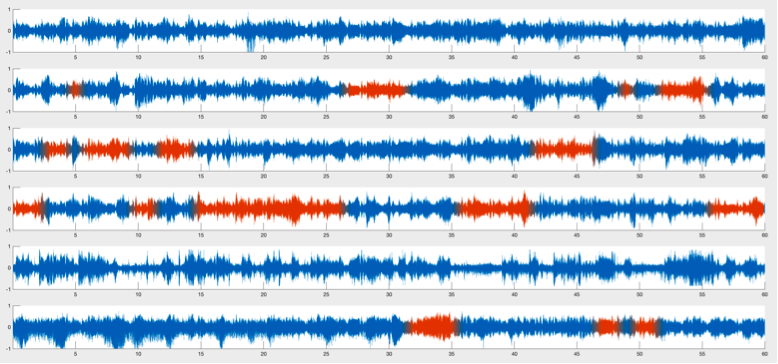
\includegraphics[width=0.8\textwidth]{switching-result1}
}
\vspace{0.8ex}
\\
\subcaptionbox{实验B实例组2} {
    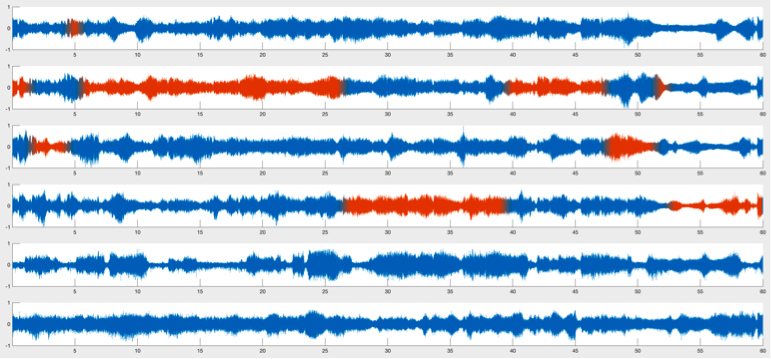
\includegraphics[width=0.8\textwidth]{switching-result2}
}
\caption{实验B输出结果波形\label{fig:switching-result}}
\end{figure}

\begin{figure}
\centering
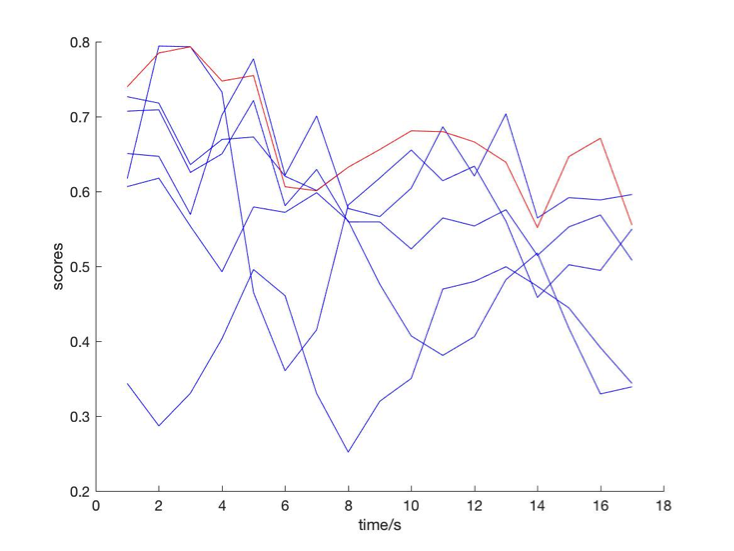
\includegraphics[width=0.45\textwidth]{switching-scores1}
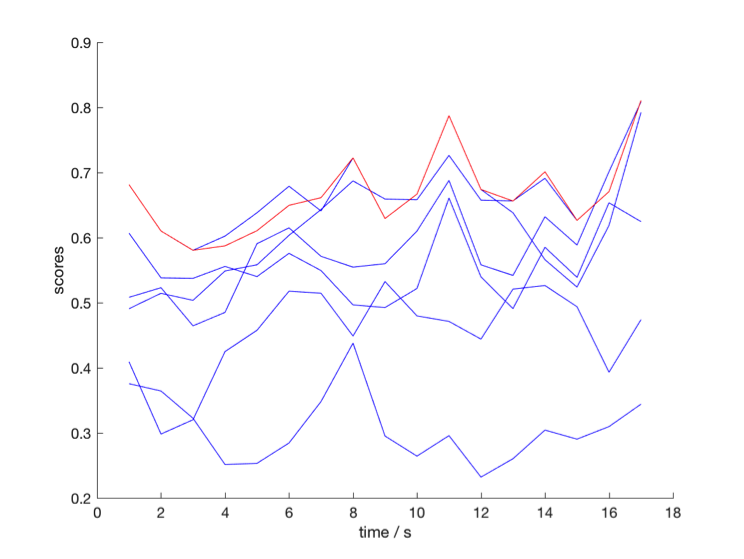
\includegraphics[width=0.45\textwidth]{switching-scores2}
\caption{实验B输出的评分结果\label{fig:switching-scores}}
\end{figure}

对每一组实验结果,我们试听了选路输出的语音和每一路原始语音,比较其主观感受质量。选路输出的语音质量整体要优于各路原始语音信号。我们也试用了客观评分算法对合路语音以及各路语音分时间段进行了客观质量评分,结果如图~\ref{fig:switching-scores}所示。其中红色折线为对选路输出的语音进行评分的结果,而蓝色折线则为各路原始语音的评分结果,从算法客观评分结果来看选路输出的语音质量也是整体最优的。

\section{小结}

本章用实验验证了本文所提算法和系统的效果。实验A中通过分析算法给出的客观评分和人给出的主观评分之间的相关性,验证了本文所提的语音质量客观评价算法在短波语音上有很好的表现。并且我们比较了本文所提算法和两种标准评分算法的结果,诸多指标表明我们的算法在短波语音上有更优秀的表现。实验B中使用本文设计的自动选路系统,对实际多地点接收的短波语音信号进行选路,验证了本文所提系统的功能。实验表明选路输出的语音质量比各路原始语音要好,达到了预想的效果。